

\section{\OurMethod: Model-Based Planning for Web Agents}
\label{sec:method}

\subsection{Preliminary}
\label{sec:planning}
Web agents tasked with automating activities in live websites face vast and complex search spaces. Formally, each task, given an instruction $I$, can be formulated as a partially observable Markov decision process (POMDP): $(\mathcal{S}, \mathcal{A}, \mathcal{O}, T, R, \Omega)$, where $\mathcal{S}$ is the set of possible environment states, $\mathcal{O}$ is the set of observations available to the agent, and $\mathcal{A}$ represents actions such as clicking elements, entering text, or navigating URLs.
$T: \mathcal{S} \times \mathcal{A} \to \mathcal{S}$ is the state transition function, while $R$ is a binary reward indicating task completion.
Due to partial observability, the agent perceives only observations $o = \Omega(s)$.
% which may be screenshots or text-based accessibility trees. 

Tree search-based planning with real interactions is costly and risks irreversible actions.
Model-based planning through simulation mitigates this by using a learned simulation function $\texttt{sim}(o, a)$ to predict outcomes before execution.
This enables online planning, where the agent iteratively selects actions based on simulated future trajectories.
A common approach is Model Predictive Control (MPC;~\cite{garcia1989model}), which simulates possible future states for each action over a finite horizon $H$, evaluates them using a scoring function $\texttt{score}(\tau)$, and executes the action with the highest score.
% : $a^* = \argmax_{a \in \mathcal{A}} \texttt{score}(\texttt{sim}(o, a))$
This process repeats after observing new states, allowing adaptive decision-making while avoiding unnecessary interactions.


\begin{figure}
    % \vspace{-0.5em}
    \centering
    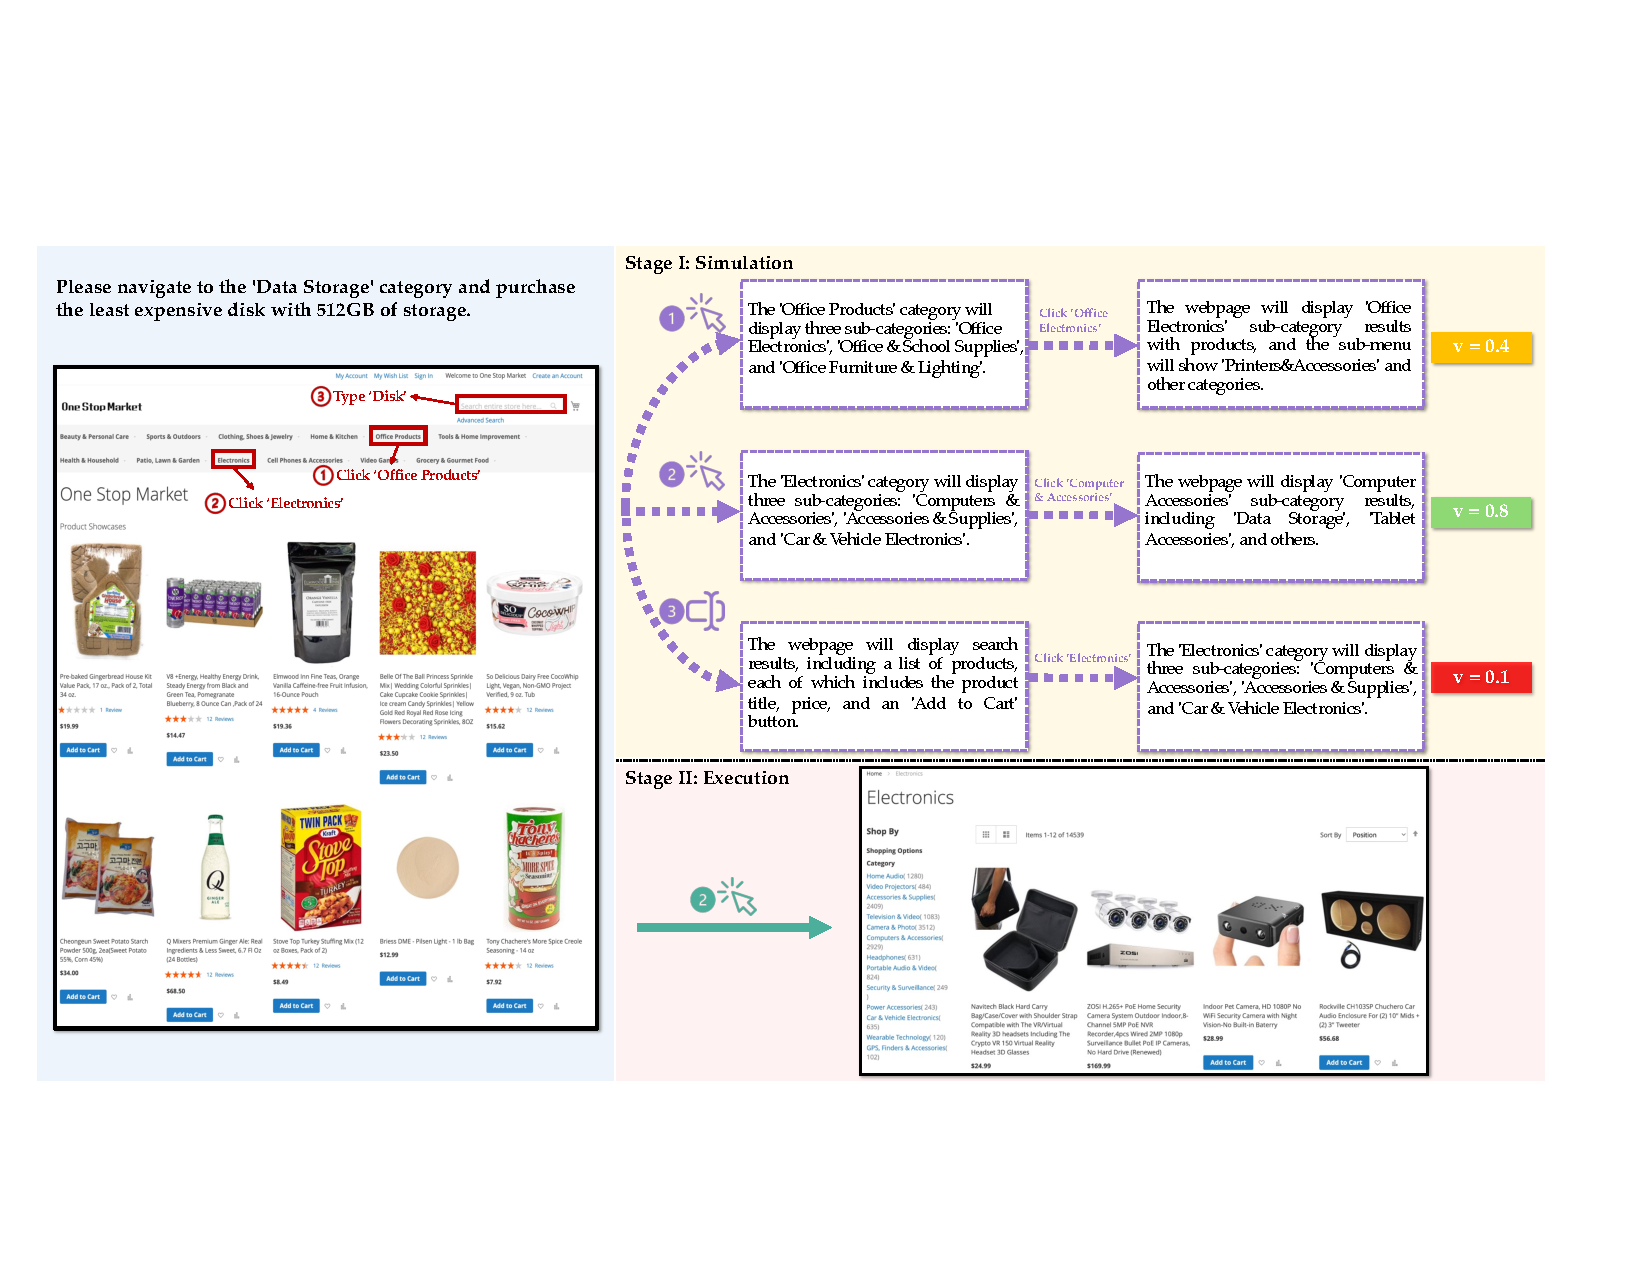
\includegraphics[width=\linewidth]{figs/wm_fig2.pdf}
    % \vspace{-0.5em}
    \caption{
     Illustration of \OurMethod simulating outcomes for three candidate actions using GPT-4o: (1) \textit{Click "Office Products"}, (2) \textit{Click "Electronics"}, and (3) \textit{Type "Disk" into textbox}.
     Each dotted box shows an LLM-generated state after a proposed action.
     Simulated trajectories are scored to identify the best action, and the optimal action \textit{Click "Electronics"} with the highest score ($v=0.8$) is executed.
     This example shows a two-step planning horizon.
     In practice, \OurMethod simulates multiple trajectories per action to capture a wider range of possible outcomes, improving coverage and leading to better-informed decisions.
     Here we only show one trajectory for each action and the final score for brevity.
    }
    \label{fig:diagram}
    % \vspace{-1.5em}
\end{figure}



\subsection{Core Design}
\label{subset:core-design}
\OurMethod follows the planning through simulation paradigm introduced in Section~\ref{sec:planning}. 
Figure~\ref{fig:diagram} illustrates this process with three candidate actions, where \OurMethod simulates two-step trajectories for each action, selects the trajectory with the highest score, and executes its corresponding initial action.
At its core, \OurMethod leverages LLMs to implement both the simulation function (\texttt{sim}) and the scoring function (\texttt{score}).

\begin{wrapfigure}{r}{0.45\textwidth}
\vspace{-1.5em}
    \centering
    \small
    \resizebox{0.45\textwidth}{!}{ 
        \begin{algorithm}[H]
            \caption{\OurMethod}
            \label{alg:planning}
            \SetAlgoLined
            \KwIn{Instruction $I$; initial observation $o_0$}
            \KwOut{Sequence of actions $a_0, a_1, \ldots, a_T$}
            $t\leftarrow 0$\;
            \While{True}{
                $\mathcal{A}_t\leftarrow \text{\texttt{get\_candidate}}(I, o_t)$\;
                $\mathcal{A}_t'\leftarrow \text{\texttt{self\_refine}}(\mathcal{A}_t)$\;
                $a_t = \argmax_{a \in \mathcal{A}_t'} \text{\texttt{score}}(\text{\texttt{sim}}(o_t, a))$\;
                $o_{t+1} \leftarrow \texttt{execute}(a_t)$\;
                $t \leftarrow t+1$\;
                \If{\texttt{termination\_check()} = True}{
                    break;
                }
            }
        \end{algorithm}
    }
    \vspace{-2em}
\end{wrapfigure}

\textbf{Implementation for \texttt{sim}.}
Our implementation of \texttt{sim} consists of two modules: one predicts state changes after action execution, approximating the state transition function $T$, while the other imagines a possible action based on the predicted state to enable long-horizon planning.
Together, these two modules generate trajectories of length $H$, where $H$ is a configurable parameter (the simulation depth).
Specifically, to represent the state changes, we prompt an LLM (GPT-4o or self-trained world models) to generate a concise natural language description focusing only on the effects of the action, as shown in Figure~\ref{fig:diagram} Stage I.

\textbf{Implementation for \texttt{score}.}
After collecting a trajectory $\tau_i$ simulated from each candidate action $a_i$ using \texttt{sim}, we further use an LLM as a scoring function for each simulation.
Following~\cite{koh2024tree}, we prompt GPT-4o to score each simulated trajectory with a three-scale response---complete (1.0), on track (0.5), or incorrect (0)---indicating its progress toward task completion. 
The final score for each action is averaged over multiple simulated trajectories and scorings, then used to determine the optimal action to execute (\eg, Click ``Electronics''), as shown in Stage I of Figure~\ref{fig:diagram}.


In addition to \texttt{sim} and \texttt{score}, a prerequisite to planning is candidate action generation.
We employ a two-stage approach: first sampling top-k actions following~\cite{koh2024tree}, then using LLM to self-refine unnecessary actions for simulation. 
This self-refinement step is motivated by our observation that at different steps, the same k can introduce varying degrees of irrelevant actions---some steps naturally have fewer plausible actions than others.
We show the pseudo code of \OurMethod's overall design in Algorithm~\ref{alg:planning}.
\texttt{termination\_check} verifies if the model outputs a \texttt{stop} action, reaches max steps, or repeats an action over 3 times, also following the implementation by~\cite{koh2024tree}. Please refer to Appendix~\ref{appendix:prompts} for more implementation details.




\subsection{World Model Data Synthesis and Model Training}
\label{subsec:train-world-model}


\begin{figure*}[tbh]
    \centering
    % \vspace{-1em}
    
\includegraphics[width=\linewidth]{figs/workflow.pdf}
    % \vspace{-0.8em}
    \captionof{figure}{Data synthesis pipeline. The pipeline consists of (1) Web Random Walking, where we autonomously interact with web pages through actions like typing for search and clicking, and (2) Synthesis, where Qwen2-VL-72B~\citep{Wang2024Qwen2VL} generates textual descriptions of state changes based on visual snapshots before and after actions.}
    \label{fig:data-construction}
    % \vspace{-0.5em}
\end{figure*}

While general-purpose LLMs such as GPT-4o have the potential to serve as world models, their cost and latency may limit their feasibility for real-time planning.
To explore a more deployable alternative, we also aim to train a small world model that offers lower inference cost and easier adaptation to new domains.

As shown in Figure~\ref{fig:data-construction}, we develop a scalable data synthesis pipeline that autonomously interacts with web pages using heuristic guidance.
We sample starting URLs from the October 2024 Common Crawl Index\footnote{https://commoncrawl.org} and perform random web actions, including clicking elements, hovering, typing into text boxes, and selecting options.
To better reflect human interaction distributions, we adjust action probabilities---favoring frequent interactions like clicking while ensuring sufficient coverage of others.
Additionally, we encourage causal dependencies by prioritizing actions on newly emerged elements, such as clicking a button that appears after hovering over a dropdown.
For search-related text inputs, we generate contextually relevant queries using GPT-3.5-turbo.

Once an interaction is performed, we capture visual snapshots before and after the action.
We then prompt Qwen2-VL-72B~\citep{Wang2024Qwen2VL} to generate textual descriptions detailing the changes in the webpage state (Figure~\ref{fig:data-construction} Step 2), ensuring an accurate representation of how each action impacts the visual content.
Each training instance consists of the initial visual state, the action taken, and the generated textual description of the state change.
After data collection, we filter out failed interactions, automation-blocked content, and potentially harmful data, resulting in a final dataset of over 3.1M interaction instances that capture rich causal relationships between user actions and web state transitions.

As we empirically find horizon step $H{=}1$ to be the most effective and efficient configuration, we focus on training the state transition function in \texttt{sim}, initializing it with Qwen2-VL-7B~\citep{Wang2024Qwen2VL}.
The final model, Dreamer-7B, is trained to predict the next state as a natural language description after performing an action on the current state, using a next-token prediction objective.
To efficiently monitor the progress of self-trained world models without relying on costly downstream evaluations for every checkpoint, we construct an intrinsic evaluation set for checkpoint selection, detailed in Appendix~\ref{appendix:intrinsic-eval}.
Appendix~\ref{appendix:data-synthesis-and-training} provides additional details on data synthesis and training.

